\chapter{Discussion}
\section{Water Year 2019} 
\subsection{Isothermal Snowpack and Runoff Timing}
In order to have considerable snowmelt runoff, there are three basic phases a snowpack must go through (warming, ripening, and output). Once the snowpack is isothermal, it enters the ripening phase where absorbed energy is used to melt snow. Although absorbed energy is used to melt snow, it is important to note that the majority of melt water is retained in the snowpack via surface tension and continuous pores filled with air. After the snowpack is fully saturated with liquid water, then it is in the output phase where further absorption of energy produces water output. It is important to note that this is a very idealized sequence. For example, melting often occurs at the surface before the ripening phase and may percolate deeper into the snowpack where it can refreeze and form ice layers. Latent heat exchange during these phase changes is not a negligible in the overall energy balance and snowpack processes. 

The SNOTEL network is currently the most robust system for measuring snowpack characteristics and it creates hourly reports of snow depth, snow water equivelence (SWE), and precipitation across the Western United States. Using snow depth and SWE to calculate snow density, it is possible to estimate when a snowpack has reached ripe conditions and this is usually around 500 kg m\textsuperscript{-3}. The current network lacks the ability to measure snowpack temperature conditions, therefore it is very hard to predict the beginning of the ripening phase. In a scenario with a lower density snowpack in its ripening phase, the current SNOTEL network doesn't provide the data necissary to make predictions on when the snowpack will enter the output phase. Combining data from the SNOTEL network, weather forecasts, and snowpack temperature arrays could provide a means to estimate the timing of the output phase. Below are foundational equations that could be used to approach this problem. 

From empirical studies, the maximum volumetric water content ($\theta$\textsubscript{ret}) that a snowpack can retain against gravity is: 
\begin{equation}
\theta \textsubscript{ret} = -0.0745\frac{\rho \textsubscript{s}}{\rho \textsubscript{w}}
+ 0.00267\frac{\rho \textsubscript{s}}{\rho \textsubscript{w}}^2 
\end{equation}
Where $\rho \textsubscript{s}$ and $\rho \textsubscript{w}$ are the densities of snow and water respectively. Ripe snowpacks usually have a bulk density of $\rho_s$ = 500 kg m\textsuperscript{-3} and according to the above equation, this leads to a maximum volumetric water content of $\theta$\textsubscript{ret} = 0.03. The net energy (Q\textsubscript{m2}) in J m\textsuperscript{-2} required to complete the ripening phase is: 
\begin{equation}
Q_{m2} = \theta_{ret} * h_s * \rho_w * \lambda_f
\end{equation}
Where h\textsubscript{s} is snow depth and $\lambda_f$ is the latent heat of fusion (0.334 MJ kg\textsuperscript{-1}). 

Using weather forecasts, it is possible to estimate the potential net energy exchange between the snowpack and atmosphere. If there is a net energy exchange into the snow that exceeds Q\textsubscript{m2}, the snowpack will likely enter the output phase. 

\begin{figure}
    \centering
    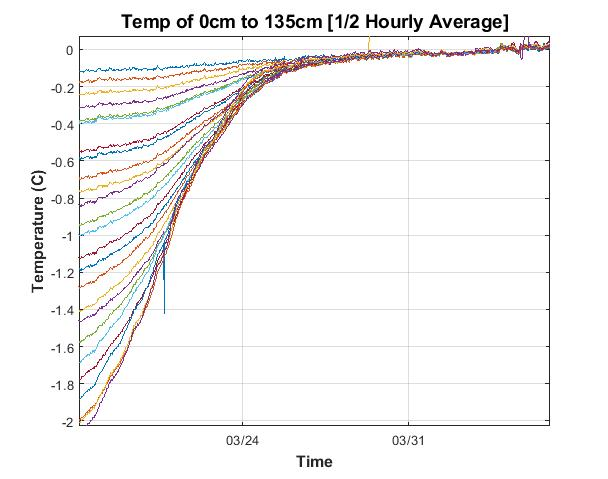
\includegraphics[width=0.7\linewidth]{figures/0_135cm_Isothermal.jpg}
    \caption{Progression of snowpack temperatures leading to isothermal conditions.}
    \label{fig:0_135cm_Isothermal}
 \end{figure}
 
 \begin{figure}
    \centering
    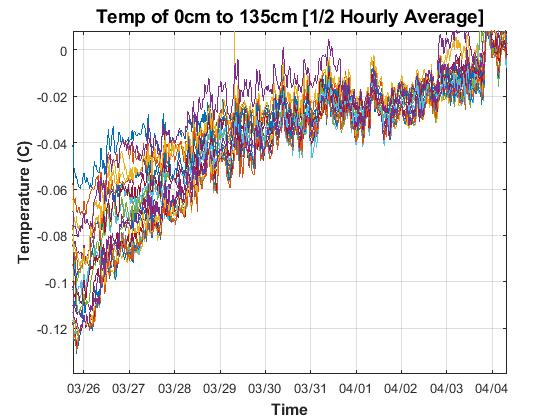
\includegraphics[width=0.7\linewidth]{figures/0_135cm_zoom.jpg}
    \caption{Sub-plot of data shown in Figure \ref{fig:0_135cm_Isothermal}}
    \label{fig:0_135cm_Zoom}
 \end{figure}

\begin{figure}
    \centering
    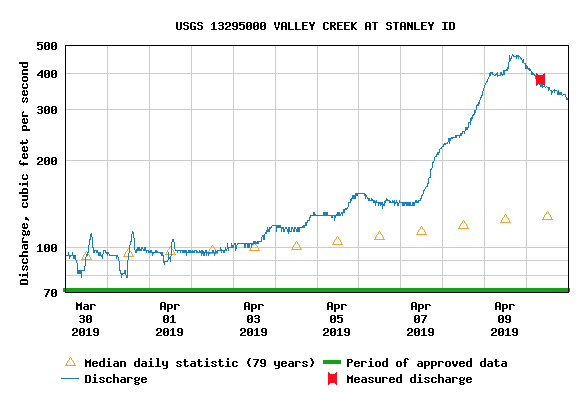
\includegraphics[width=0.8\linewidth]{figures/ValleyCreek_Gage.png}
    \caption{\textbf{Valley Creek} Unregulated streamflow data from a USGS gage near Banner Summit.}
    \label{fig:ValleyCreek}
 \end{figure}

\subsection{Temperature Gradient Metamorphism}
Temperature-gradient metamorphism is the process of vapor transport along a thermal gradient (\cite{sommerfeld_1970}). As long as the gradient is maintained, as is usually the case in cold environments, the process continually acts on the snowpack. The snow characteristics during the beginning of this process have a strong effect on its progress (\cite{sommerfeld_1970}). In new, fine grained, porous snow, there are more grains in which the diffusing vapor can freeze. Resulting, the grains do not grow very large, and hollow pyramids are not common (\cite{sommerfeld_1970}). If temperature-gradient metamorphism starts in larger-grained, equi-temprature metamorphosed snow, there are fewer crystals on which the vapor can freeze. Under a consistent thermal gradient, these crystals will grow larger, and hollow pyramids along with lattice grains may be found (\cite{akitaya_1967}). 



\subsection{Comparison to a Model}

\subsection{Stable Water Isotopes}
The 2019 isotope data have some significant random error because samples were taken in a lightly forested area with varying amounts of underbrush and fallen trees. This uneven ground creates an inconsistent datum between sampling events and introduces an unexpected amount of spatial variability. In addition to this, stable water isotopes could be effected by nearby trees and buried brush that emit longwave radiation. Moving forward, sampling for stable water isotopes in snow should be conducted open areas with an even ground surface that is free of large brush, or fallen debris. If a study is conducted in a forested/lightly forested area, there should be a preseason effort to clear the sampling locations of anything that makes the sampling locations uneven. 

- Interpretability of WY2019 isotope dataset \\
- Future directions  \\
- Coupling temperature and isotope dataset \\
